\section{Arquitectura del Servidor}
\begin{figure}[!htb]
    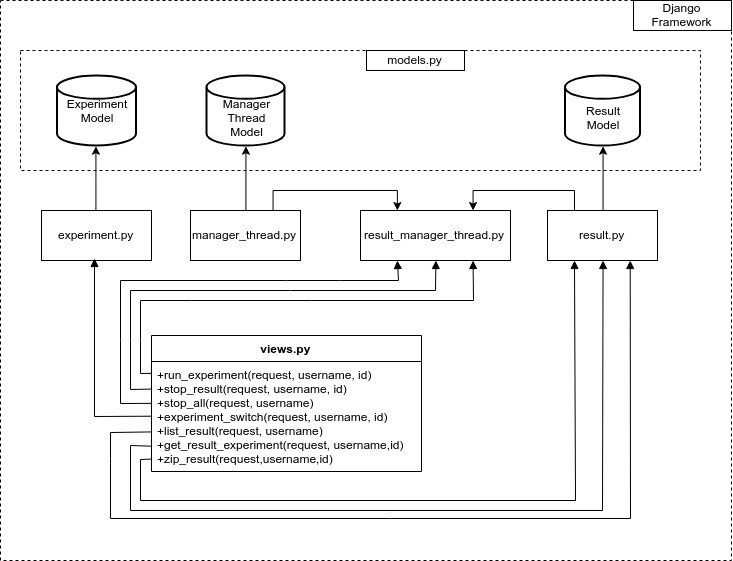
\includegraphics[width=\linewidth]{../figures/d20.jpg}
    \caption{Arquitectura del Servidor}
    \label{fig:d20}
\end{figure}

El \textit{Servidor} cumple con la estructura que propone \textit{Django Framework} siguiendo el 
patr\'on MVC\cite{django_tutorial}. En este proyecto existen 3 modelos b\'asicos que abstraen el experimento, resultados
y ejecuci\'on del mismo para el seguimiento del estado de un experimento en curso.
Cada modelo tiene una abstracci\'on intermedia con la finalidad de ofrecer las operaciones sobre
los estos cumpliendo los requerimientos de usuario para ser invocados por los servicios REST implementados
en las vistas.

\newpage